% 'draft' mode can be used to speed up compilation
\documentclass[twoside,final]{Contexto}
\usepackage{codespace}

% Draft watermark
% https://github.com/callegar/LaTeX-draftwatermark

% Encodings
\usepackage{gensymb,textcomp}

% Better tables
% Wide tables go to https://tex.stackexchange.com/q/332902
\usepackage{array,longtable,multicol,multirow,siunitx,tabularx}

% Better enum
\usepackage{enumitem}

% Graphics
\usepackage{caption,float}

% Add options for figures, like max width, framing, etc.
\usepackage[export]{adjustbox}

% References
% Use \Cref{} instead of \ref{}
\usepackage[nameinlink]{cleveref}

% FOR DEMONSTRATION PURPOSES, REMOVE IN PRODUCTION
\usepackage{mwe}


\usepackage[acronym]{glossaries} % For acronyms in acronyms.tex
\makeglossaries
\newacronym{ai}{AI}{artificial intelligence}
\newacronym{ml}{ML}{machine learning}
\newacronym{hcai}{HCAI}{human-centered artificial intelligence}
\newacronym{hgml}{HGML}{human-guided machine learning}
\newacronym{automl}{AutoML}{automated machine learning}
\newacronym{llm}{LLM}{large language model}
\newacronym{aws}{AWS}{amazon web services}
\newacronym{rag}{RAG}{retrieval‑augmented generation}
\newacronym{crp}{CRP}{clinical research professional}
\newacronym{hamelin}{HAMELIN}{Human-guided Automated Machine Learning for Clinical Studies}
\newacronym{gui}{GUI}{graphical user interface}
\usepackage{tikz}
\usetikzlibrary{shadows}
\usetikzlibrary{positioning}

\usepackage{graphicx}   % resizebox
\usepackage{booktabs}   % \toprule, \midrule, \bottomrule
\usepackage{multirow}   % \multirow
\usepackage{amssymb}    % \checkmark


% Sub-preambles
% https://github.com/MartinScharrer/standalone

% Configurations
\coursename{Convocatoria 2023\\ «Proyectos de Generación de Conocimiento» y actuaciones\\ para la formación de personal investigador predoctoral\\ asociadas a dichos proyectos.}
\reporttype{}
\title{Human-guided Automated Machine Learning for Clinical Studies (HAMELIN)}
\advisor{& Rafael Duque Medina &}

% Allow page breaks inside align* environment
%\allowdisplaybreaks{}

% Makes a lot of things blue, avoid at all costs
%\everymath{\color{blue}}

% Set depth of numbering for counters
\AtBeginDocument{\counterwithin{lstlisting}{section}}

% Rename some sections
%\AtBeginDocument{\renewcommand*{\contentsname}{Contents}}
%\AtBeginDocument{\renewcommand*{\refname}{References}}
%\AtBeginDocument{\renewcommand*{\bibname}{References}}

% Custom commands
%\newcommand*\mean[1]{\bar{#1}}

% Allow page breaks inside align* environment
%\allowdisplaybreaks{}

% Makes a lot of things blue, avoid at all costs
%\everymath{\color{blue}}

% Set depth of numbering for counters
\AtBeginDocument{\counterwithin{lstlisting}{section}}

% Rename some sections
%\AtBeginDocument{\renewcommand*{\contentsname}{Contents}}
%\AtBeginDocument{\renewcommand*{\refname}{References}}
%\AtBeginDocument{\renewcommand*{\bibname}{References}}

% Custom commands
%\newcommand*\mean[1]{\bar{#1}}
\AtBeginDocument{\renewcommand{\contentsname}{Content}}
\AtBeginDocument{\renewcommand{\listfigurename}{Figure list}}
\AtBeginDocument{\renewcommand{\listtablename}{Table list}}
\AtBeginDocument{\renewcommand{\tablename}{Table}}
\AtBeginDocument{\renewcommand{\figurename}{Figure}}
\AtBeginDocument{\renewcommand{\refname}{Reference}}

\begin{document}
\coverpage%

%\section*{Member list \& Workload}
%\newcounter{memberrowno}
%\setcounter{memberrowno}{0}
%\begin{center}
%  \begin{tabular}{>{\stepcounter{memberrowno}\thememberrowno}llcc}
%    \toprule
%    \multicolumn{1}{c}{\textbf{No.}} & \textbf{Full name} & \textbf{Student ID} & \textbf{Contribution} \\
%    \midrule
%                                     & h                  & xxxxxxx             & 100\%                       \\
%                                     & h                  & xxxxxxx             & 100\%                       \\
%    \bottomrule
%  \end{tabular}
%\end{center}
%\clearpage

\tableofcontents
\listoffigures
\listoftables
\lstlistoflistings{}

\clearpage

\section{State of the art}
\label{sec:state-of-the-art}

This section reviews the main strands of research underpinning this work. First, it examines existing \gls{automl} solutions, distinguishing between commercial and free tools. It then introduces the principles of \gls{hcai}, which argue for placing people at the center of \gls{ai} systems. Finally, it presents \gls{hgml} as a practical approach that integrates \gls{hcai} principles into the design and use of \gls{ml} workflows.

\subsection{AutoML tools}
\label{subsec:automltools}

The rapid expansion of \gls{ml} applications in the mid‑2010s, combined with a shortage of specialized data scientists, created a strong need for tools that could reduce the technical barrier to entry \cite{he2021automl}. \gls{automl} tools emerged in this context with a clear ambition: to democratize \gls{ml}. They do so by automating tasks that traditionally required expert knowledge, such as feature engineering, model selection, hyperparameter tuning and, deployment.

The aim of \gls{automl} is therefore to lower the time, expertise and infrastructure requirements associated with building accurate \gls{ml} models. This allows domain experts, who may not be specialists in \gls{ml}, to take advantage of \gls{ai} methods for decision-making and problem-solving. By offloading repetitive and labor‑intensive operations to the system, both novice users and experienced practitioners can dedicate more effort to defining the problem, specifying constraints and interpreting results. As a consequence, \gls{automl} has played a key role in facilitating the broader diffusion of \gls{ml} across sectors such as finance, healthcare, marketing and industry. The current landscape comprises a wide variety of tools, from commercial products to open and free alternatives, each targeting different user profiles and project scales.

\subsubsection{Commercial tools}

Among commercial offerings, major cloud providers and specialized \gls{ml} platforms dominate the \gls{automl} market. These solutions typically integrate tightly with existing cloud services and seek to support the entire \gls{ml} lifecycle.

Within the Google Cloud ecosystem, Google AutoML \cite{GoogleAutoML} provides dedicated services for computer vision, natural language processing and tabular data. It relies heavily on graphical interfaces and smooth integration with other Google services, which facilitates adoption by users with limited \gls{ml} experience. Similarly, Azure Automated ML \cite{AzureAutomatedML} concentrates on tabular data and time-series forecasting, but distinguishes itself through a strong emphasis on model explainability and interoperability with Microsoft tools such as Power BI. This focus on interpretability and integration is particularly valuable in sectors subject to strict regulatory requirements. On the \gls{aws} side, Amazon SageMaker Autopilot \cite{AmazonSagemakerAutopilot} automates the construction and training of models for tabular data, providing explainable models and the ability to inspect and customize the generated code. Its pay-as-you-go pricing and alignment with the broader \gls{aws} ecosystem make it attractive for organizations of different sizes, especially in applications such as customer analytics and fraud detection.

Beyond general-purpose cloud services, a number of specialized platforms offer advanced features targeted at enterprise use cases. DataRobot \cite{DataRobot} exemplifies this trend, with strong support for explainability, security and regulatory compliance that make it appealing for banks, insurance companies and healthcare organizations. H2O.ai’s Driverless AI \cite{DriverlessAI} combines wide coverage of \gls{ml} tasks—including time-series forecasting—with sophisticated interpretability mechanisms. Other tools, such as Auger.AI \cite{AugerAI}, prioritize high predictive performance and seamless API integration, while Darwin \cite{Darwin} focuses on accelerating workflow development with accessible interfaces for both novices and advanced users. Some systems are tailored to specific domains: JADBio \cite{JADBio}, for example, is oriented toward molecular biology data. In addition, long‑standing platforms such as BigML \cite{BigML} and RapidMiner \cite{RapidMiner} provide mature, user‑friendly environments, and IBM Watson AutoAI \cite{Watson} benefits from its seamless fit with IBM’s enterprise ecosystem.

Despite the richness of these commercial solutions, high licensing and infrastructure costs remain a major obstacle for many academic groups and independent practitioners. This limitation has motivated the use and development of free \gls{automl} alternatives.

\subsubsection{Free tools}
\label{subsubsec:free_tools}

Free \gls{automl} frameworks play a crucial role in widening access to advanced \gls{ml} methods, particularly for research teams and practitioners without large software budgets. They make it possible to experiment with state‑of‑the‑art techniques without incurring licensing costs. From the many available tools, the most widely adopted ones were selected for closer examination \cite{palazuelos2024non}.

Some tools are oriented toward data integration and knowledge management. MindsDB \cite{mindsdb}, for instance, can be seen as a query engine that unifies disparate data sources behind SQL interfaces. This capability makes it suitable for building \gls{rag} systems and knowledge bases.

Other frameworks address more specific modeling tasks. Prophet \cite{prophet}, developed by Meta, is specialized in time-series forecasting. It uses additive models that explicitly incorporate seasonality and holiday effects and is designed to be robust in the presence of missing data and abrupt trend changes. H2O-3 \cite{h2o3}, in contrast, is a general-purpose library that focuses on supervised learning. It combines fast random search with stacked ensembles to obtain competitive performance and integrates smoothly with big data infrastructures such as Hadoop and Spark.

A second group of tools centers on hyperparameter optimization and neural architecture search. NNI \cite{nni} (from Microsoft) offers flexible \gls{automl} functionality for hyperparameter tuning, architecture search and model compression, configured through Python and YAML. Optuna \cite{optuna} provides a highly efficient, parallelizable hyperparameter optimization framework that can be used with multiple backends, while Hyperopt applies Bayesian optimization to guide the search process. Auto-Sklearn \cite{autosklearn} works as a drop‑in replacement for Scikit‑learn and combines Bayesian optimization, meta-learning and ensemble construction to improve model performance with minimal code changes.

A third category of tools focuses on automating entire pipelines. Ludwig \cite{ludwig} adopts a declarative approach: users specify deep learning pipelines for tabular data, natural language processing and computer vision through YAML configuration files rather than imperative code. PyCaret \cite{pycaret} and AutoGluon \cite{autogluon} (from \gls{aws}) support rapid experimentation and prototyping, providing low‑code interfaces that automate preprocessing, feature engineering and evaluation. TPOT \cite{tpot} explores large spaces of candidate pipelines using genetic programming and ultimately produces Python code corresponding to the best discovered solutions. AutoKeras \cite{autokeras}, built on top of Keras, focuses on simplifying model selection, hyperparameter tuning and validation via Python code, but interpreting the resulting models still demands technical expertise. Featuretools \cite{featuretools} automates feature engineering for temporal and relational data, generating useful structured features with relatively little coding effort, although domain knowledge remains essential for making sense of the results.

Taken together, these tools illustrate the diversity of the free \gls{automl} ecosystem. Some frameworks emphasize usability, for example by providing graphical interfaces or high‑level abstractions, but may compromise on configurability or depth of automation. Others prioritize flexibility and optimization capabilities while offering fewer interactive or interpretability-oriented features. In practice, the most appropriate tool depends on the specific trade-offs and priorities of each research or application context.

\subsection{Human-Centered Artificial Intelligence}
\label{subsec:hcai}

The growth of \gls{ai} systems capable of impacting critical aspects of society has prompted a rethinking of how such systems should be designed. \gls{hcai} has emerged as a response to this challenge. Instead of focusing solely on improving algorithmic performance, the \gls{hcai} perspective places humans at the center of the entire lifecycle of \gls{ai} systems \cite{shneiderman2022human}.

In this view, \gls{ai} should not replace people, but rather amplify, augment and empower them. Interfaces and interactions are therefore not secondary concerns; they are essential for ensuring that users retain meaningful control over automated processes. This shift is reflected in what is sometimes described as a ``third wave'' of \gls{ai}, in which advances in algorithms and computing are combined with human-centered design practices. In this context, human-computer interaction specialists and \gls{ai} researchers share responsibility for creating systems that are not only powerful but also ethical, comprehensible and practically useful \cite{xu2019toward}.

Traditional \gls{ai} systems, despite their impressive performance, pose several risks. Bias is one of the most pressing issues: if training data are unbalanced or unrepresentative, the resulting models may reproduce or amplify unfair patterns in decisions. A second major concern is opacity. Many high-performing models behave as ``black boxes'', making it difficult for users to understand the reasons behind particular outputs or to detect when the system is failing. \gls{hcai} explicitly addresses these problems by encouraging practices such as systematic bias identification, the design of interfaces that allow users to explore and influence model behavior, the use of explainable \gls{ai} techniques to improve transparency and the incorporation of human oversight in high‑stakes scenarios \cite{chen2023human}.

Although the ideas behind \gls{hcai} are now widely discussed in research, their translation into concrete industrial practices and methods has been slower. One of the reasons is the lack of detailed methodological guidance on how to operationalize human-centered principles in everyday design and development work \cite{hartikainen2022human}. To help bridge this gap, a specific \gls{hcai} framework has been proposed.

Conventional discussions of automation typically rely on the notion of ``levels of autonomy'', which assumes a simple trade‑off: as automation increases, human control decreases, and vice versa. Full autonomy is associated with systems that make all decisions independently, whereas minimal autonomy implies that humans are responsible for every step. The \gls{hcai} framework challenges this view by decoupling automation from human control. Instead of treating them as opposite ends of a single continuum, it treats them as two separate dimensions that can be simultaneously high. This leads to a two‑dimensional conception in which the goal is not to maximize automation at the expense of users, but to design systems that are both highly automated and strongly controllable.

Figure \ref{fig:HCAI_dimensions} illustrates this idea. The horizontal axis captures the degree of computer automation, and the vertical axis captures the level of human control. The lower-left quadrant corresponds to simple systems with little automation and limited human influence. The upper-right quadrant corresponds to the ideal target of the framework: systems in which automation is extensive, yet people still retain meaningful, well-supported control over key decisions. The remaining quadrants represent intermediate situations in which one of the dimensions is high and the other low.

\begin{figure}[H]
\centering
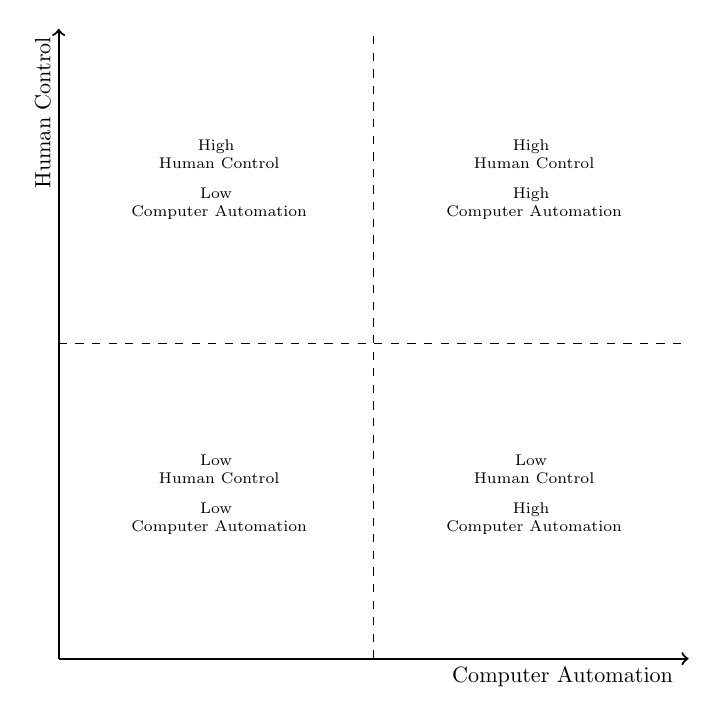
\begin{tikzpicture}[scale=0.8, transform shape]
    % Set axis limits
    \draw[->, thick] (0,0) -- (10,0) node[anchor=north, xshift=-2cm] {Computer Automation};
    \draw[->, thick] (0,0) -- (0,10) node[anchor=south east, rotate=90] {Human Control};

    \draw[dashed] (0,5) -- (10,5); % Horizontal division
    \draw[dashed] (5,0) -- (5,10); % Vertical division

    \node[align=center, font=\scriptsize] at (2.5,2.5) {Low \\ \vspace{0.2cm} Human Control \\ Low \\ \vspace{0.2cm} Computer Automation};
    \node[align=center, font=\scriptsize] at (7.5,2.5) {Low \\ \vspace{0.2cm} Human Control \\ High \\ \vspace{0.2cm} Computer Automation};
    \node[align=center, font=\scriptsize] at (2.5,7.5) {High \\ \vspace{0.2cm} Human Control \\ Low \\ \vspace{0.2cm} Computer Automation};
    \node[align=center, font=\scriptsize] at (7.5,7.5) {High \\ \vspace{0.2cm} Human Control \\ High \\ \vspace{0.2cm} Computer Automation};
\end{tikzpicture}
\caption{Two-dimensional HCAI framework}
\label{fig:HCAI_dimensions}
\end{figure}

To make this framework operational in the context of \gls{automl}, 13 free tools were analyzed according to the two dimensions. Table \ref{tab:HCAIframework} summarizes the results. For each tool, it considers three indicators of human control, ease of use, pipeline configurability and interpretability of outputs, and six indicators of automation—data type handling, data cleaning, feature engineering, model training, hyperparameter tuning and model validation.

In terms of human control, ease of use ranges from technically demanding tools that require programming skills to interfaces that support non-experts through drag-and-drop or guided workflows. Configurable pipeline captures the flexibility to adjust steps in the workflow, from rigid, predefined sequences to pipelines that can be customized in detail. Interpretable information reflects how accessible and understandable the outputs are, from raw technical logs to dashboards and visual explanations in more natural language.

The automation dimension evaluates how much of the end‑to‑end process a tool can manage without human intervention. It includes the automatic identification of data types, built‑in preprocessing and cleaning, automated feature construction, training across multiple algorithms, hyperparameter optimization routines and systematic validation procedures. High scores on these indicators suggest that a tool can handle large parts of the \gls{ml} lifecycle autonomously, while still leaving room for user oversight and intervention where appropriate.

\begin{table}[ht]
\centering
\scriptsize
\renewcommand{\arraystretch}{1.5}
\resizebox{\textwidth}{!}{%
\begin{tabular}{c c c c | c c c c c c}
\toprule
\multirow{3}{*}{\textbf{\begin{tabular}{@{}c@{}} AutoML \\ tool \end{tabular}}} 
  & \multicolumn{9}{c}{\textbf{HCAI Framework}} \\ \cmidrule(lr){2-10}
  & \multicolumn{3}{c|}{\textbf{Human Control}} 
  & \multicolumn{6}{c}{\textbf{High Automation}} \\ \cmidrule(lr){2-4} \cmidrule(lr){5-10}
  & \textbf{\begin{tabular}{@{}c@{}} Easy-to-use \end{tabular}} 
  & \textbf{\begin{tabular}{@{}c@{}} Configurable \\ pipeline \end{tabular}} 
  & \textbf{\begin{tabular}{@{}c@{}} Interpretable \\ information \end{tabular}} 
  & \textbf{\begin{tabular}{@{}c@{}} Data \\ types \end{tabular}} 
  & \textbf{\begin{tabular}{@{}c@{}} Data \\ cleaning \end{tabular}} 
  & \textbf{\begin{tabular}{@{}c@{}} Feature \\ engineering \end{tabular}} 
  & \textbf{\begin{tabular}{@{}c@{}} Model \\ training \end{tabular}} 
  & \textbf{\begin{tabular}{@{}c@{}} Hyperparameter \\ tuning \end{tabular}} 
  & \textbf{\begin{tabular}{@{}c@{}} Model \\ validation \end{tabular}} \\ \midrule
\textbf{MindsDB} & Medium & Low & Medium & \checkmark & \checkmark & \checkmark & \checkmark & \checkmark & \checkmark \\
\textbf{Prophet} & Low & Medium & Medium &  & \checkmark &  & \checkmark & \checkmark & \checkmark \\
\textbf{NNI} & Medium & High & Medium &  &  & \checkmark & \checkmark & \checkmark & \checkmark \\
\textbf{H2O-3} & Medium & High & Medium & \checkmark & \checkmark & \checkmark & \checkmark & \checkmark & \checkmark \\
\textbf{Ludwig} & Medium & High & Medium & \checkmark & \checkmark & \checkmark & \checkmark & \checkmark & \checkmark \\
\textbf{Optuna} & Low & High & Medium &  &  &  & \checkmark & \checkmark & \checkmark \\
\textbf{PyCaret} & Low & High & Medium & \checkmark & \checkmark & \checkmark & \checkmark & \checkmark & \checkmark \\
\textbf{TPOT} & Low & High & Low & \checkmark &  & \checkmark & \checkmark & \checkmark & \checkmark \\
\textbf{AutoKeras} & Low & High & Low &  &  &  & \checkmark & \checkmark & \checkmark \\
\textbf{AutoGluon} & Medium & High & Medium & \checkmark & \checkmark & \checkmark & \checkmark & \checkmark & \checkmark \\
\textbf{Hyperopt} & Low & High & Low &  &  &  & \checkmark & \checkmark &  \\
\textbf{Featuretools} & Low & Medium & Low &  &  & \checkmark &  &  &  \\
\textbf{Auto-Sklearn} & Low & High & Low & \checkmark & \checkmark & \checkmark & \checkmark & \checkmark & \checkmark \\ 
\bottomrule
\end{tabular}}
\caption{HCAI framework applied to AutoML tools.}
\label{tab:HCAIframework}
\end{table}

The comparison highlights distinct profiles among the tools. Frameworks such as PyCaret, Ludwig, H2O-3 and AutoGluon offer broad automation across the pipeline and, at the same time, maintain moderate levels of human control. This combination makes them attractive for research settings that demand both flexibility and efficiency. In contrast, Optuna, NNI and Hyperopt concentrate on hyperparameter optimization and neural architecture search, offering powerful configuration and optimization capabilities but with fewer features aimed at ease of use. Tools such as Featuretools and Prophet are more narrowly focused: they deliver strong automation in their respective domains (feature engineering and time-series forecasting) but do not cover the entire \gls{ml} pipeline.

Overall, the analysis shows that none of the examined tools achieves simultaneously maximum human control and maximum automation. Each solution represents a particular compromise between accessibility, interpretability and technical sophistication. This diversity reflects the evolving nature of the free \gls{automl} ecosystem and underscores the need for researchers and practitioners to choose tools based on the specific priorities of their projects. By positioning these 13 frameworks within the \gls{hcai} perspective, the analysis also reveals where current tools align with, and where they fall short of, human-centered design principles.

\subsection{Human-Guided Machine Learning}
\label{subsec:hgml}

The \gls{hcai} framework provides a conceptual basis for thinking about \gls{ai} systems that are both highly automated and under meaningful human control. \gls{hgml} can be understood as a concrete realization of these ideas in the context of \gls{ml}. Rather than fully delegating search and optimization to the system, \gls{hgml} incorporates expert knowledge into the process in a systematic way \cite{gil2019towards}.

From this perspective, \gls{hgml} offers a hybrid alternative to conventional \gls{automl}. Automated methods are still responsible for exploring model and hyperparameter spaces, but human experts actively guide this exploration. Interfaces and interaction mechanisms are therefore not merely add‑ons, but central components: they provide the channels through which experts inject domain knowledge, constraints and preferences. This combination can lead to models that are not only accurate but also more efficient and easier to interpret.

\gls{hgml} approaches emphasize expert involvement throughout the full \gls{ml} pipeline. At the data level, experts decide which features and instances to include, remove low‑quality or irrelevant data, engineer new variables and define transformations, and impose domain‑\\specific constraints. They may also segment data into subpopulations, handle outliers and design appropriate training/test splits. During model development, they influence the \gls{automl} process by selecting model families, setting priors or bounds for hyperparameters and shaping preprocessing and feature engineering strategies. This interactive guidance supports both broad exploration and targeted optimization. In the final stages, focused on evaluation and interpretation, experts use tools to inspect tailored metrics, analyze feature contributions, compare alternative models and perform sensitivity analyses to assess robustness and identify critical parameters.

However, most existing \gls{automl} systems remain strongly oriented toward maximizing predictive performance. As a result, many of them provide limited interactivity and restricted opportunities for experts to steer the process. A more human-centered approach is therefore needed to combine effectively the strengths of automated search with domain understanding \cite{lindauer2024position}. Such an approach should pursue at least five core goals: (1) high predictive performance, (2) fast optimization, (3) transparency and interpretability, (4) customizability and flexibility and (5) usability and rich interaction. While the first two goals have received significant attention in the literature, the other three, closely tied to human-centered design, remain comparatively underexplored.

% Revisar
As shown in the comparative analysis of \gls{hgml} approaches (Table \ref{tab:HGML_comparison}), existing proposals often only partially address the pipeline. Some focus on data refinement, others on model configuration or result analysis, and only rarely do they provide end‑to‑end software systems that non‑\gls{ai} specialists can use in practice. To respond to these limitations, a proposal was conceived as a framework that spans the entire pipeline and is delivered as a ready‑to‑use software implementation, aimed at integrating human guidance and automation in a consistent, practical manner.

\begin{table}[h]
\centering
\resizebox{\linewidth}{!}{%
\begin{tabular}{lcccccccccccc}
\toprule
\multirow{2}{*}{\textbf{Reference}} &
\multicolumn{3}{c}{\textbf{Data Use}} &
\multicolumn{3}{c}{\textbf{Model Development}} &
\multicolumn{3}{c}{\textbf{Model Interpretation}} &
\multirow{2}{*}{\textbf{\begin{tabular}{@{}c@{}} Software \\ support \end{tabular}}} &
\multirow{2}{*}{\textbf{\begin{tabular}{@{}c@{}} Evaluation \\ based on \\ HCAI criteria \end{tabular}}} \\ 
\cmidrule(lr){2-4} \cmidrule(lr){5-7} \cmidrule(lr){8-10} &
\textbf{\begin{tabular}{@{}c@{}} Variable \\ selection \end{tabular}} & 
\textbf{\begin{tabular}{@{}c@{}} Variable \\ requirements \end{tabular}} & 
\textbf{\begin{tabular}{@{}c@{}} Instance \\ selection \end{tabular}} & 
\textbf{\begin{tabular}{@{}c@{}} Model \\ selection \end{tabular}} & 
\textbf{\begin{tabular}{@{}c@{}} Parameter \\ settings \end{tabular}} & 
\textbf{\begin{tabular}{@{}c@{}} Solution \\ design \end{tabular}} & 
\textbf{\begin{tabular}{@{}c@{}} Model \\ assessment \end{tabular}} & 
\textbf{\begin{tabular}{@{}c@{}} Model \\ comparison \end{tabular}} & 
\textbf{\begin{tabular}{@{}c@{}} Parameter \\ comparison \end{tabular}} & & \\ 
\midrule
Gil et al. (2019) & $\checkmark$ & $\checkmark$ & $\checkmark$ & $\checkmark$ & $\checkmark$ & $\checkmark$ & $\checkmark$ & $\checkmark$ & $\checkmark$ & -- & -- \\ 
Francia et al. (2023) & $\checkmark$ & $\checkmark$ & -- & $\checkmark$ & $\checkmark$ & $\checkmark$ & $\checkmark$ & $\checkmark$ & -- & Expert-only & -- \\ 
Lee et al. (2020) & $\checkmark$ & $\checkmark$ & $\checkmark$ & $\checkmark$ & $\checkmark$ & $\checkmark$ & $\checkmark$ & $\checkmark$ & $\checkmark$ & -- & -- \\ 
Lindauer et al. (2024) & $\checkmark$ & $\checkmark$ & -- & $\checkmark$ & $\checkmark$ & $\checkmark$ & $\checkmark$ & $\checkmark$ & $\checkmark$ & -- & -- \\ 
\gls{hamelin} & $\checkmark$ & $\checkmark$ & $\checkmark$ & $\checkmark$ & $\checkmark$ & $\checkmark$ & $\checkmark$ & $\checkmark$ & $\checkmark$ & $\checkmark$ & $\checkmark$ \\ 
\bottomrule
\end{tabular}%
}
\caption{HGML approaches comparison}
\label{tab:HGML_comparison}
\end{table}



\section{Integrating CRP's competencies in the context of ML tasks}
\label{sec:crp_competencies}

The successful deployment of \gls{hgml} systems in clinical research depends critically on understanding how \glspl{crp} work with data and how their domain expertise can be systematically incorporated into \gls{ml} workflows. This section examines the specific competencies that \glspl{crp} bring to the modeling process and describes how these competencies were translated into interface design principles through an iterative, user-centered approach.

\subsection{Analysis of the most common actions involved in preprocessing data by CRPs}

Clinical research data differ fundamentally from generic datasets in their structure, semantics and regulatory constraints. \glspl{crp} routinely perform data preparation tasks that reflect deep understanding of clinical protocols, yet these tasks are rarely formalized in ways that \glspl{automl} systems can recognize or support.

\subsubsection{Protocol-aware data organization}

Clinical studies, whether patient registries, observational studies or clinical trials, impose specific organizational requirements on data. \glspl{crp} distinguish between different classes of variables according to their role in the research design. Demographic variables such as age and sex appear across virtually all studies and serve as baseline descriptors. Clinical variables such as weight, height and body mass index (BMI) are common but not universal; their relevance depends on the specific pathology under investigation. Outcome variables (endpoints) must be clearly separated from exposure variables and covariates. In clinical trials, this distinction is formalized through the protocol: primary endpoints measure efficacy, secondary endpoints assess safety, and inclusion/exclusion criteria define the study population.

Traditional \gls{automl} tools treat all columns in a dataset as equivalent candidates for feature selection. This approach ignores the semantic hierarchy inherent in clinical data. For example, a variable indicating whether a patient meets an inclusion criterion should not be used as a predictor in a model trained to forecast treatment outcomes, because it defines the population rather than describing individual variation within that population. \glspl{crp} understand these distinctions intuitively, but existing systems provide no mechanism to encode them.

\subsubsection{Temporal structure and protocol phases}

Clinical trials unfold over time in well-defined phases: screening, baseline assessment, intervention, follow-up and endpoint evaluation. Variables collected at different phases have different meanings. A blood pressure measurement taken during screening serves to determine eligibility, whereas the same measurement taken at follow-up may serve as an outcome. \glspl{crp} routinely organize data according to these temporal phases, yet \gls{automl} systems typically assume that all variables are measured simultaneously or that temporal ordering is irrelevant.

% Revisar
The meetings with \glspl{crp} revealed that temporal framing is a recurring challenge. When asked to build predictive models, \glspl{crp} need to specify not only which variables to include but also when those variables were measured relative to the outcome. This requires interfaces that allow users to define protocol phases explicitly and to assign variables to phases. Without such support, there is a risk of data leakage, using information collected after the outcome to predict that outcome, which invalidates the model.

\subsubsection{Handling missing data in clinical contexts}

Missing data are ubiquitous in clinical research. Patients may miss follow-up visits, laboratory tests may fail, or certain measurements may be contraindicated for specific individuals. \glspl{crp} assess whether data are missing completely at random (MCAR), missing at random (MAR), or missing not at random (MNAR), and choose appropriate strategies accordingly. However, most \gls{automl} systems apply generic imputation methods (mean substitution, forward filling) without considering the clinical context.

% Revisar
The analysis of \gls{crp} workflows identified several domain-specific practices. For safety variables, missing values often indicate that an adverse event did not occur, and should be coded as such rather than imputed. For longitudinal measurements, \glspl{crp} prefer to carry forward the last observed value only when clinically justified. For baseline covariates, \glspl{crp} may choose to exclude individuals with missing data rather than impute, especially when the missingness is informative. These practices reflect clinical judgment and cannot be fully automated, but they can be supported through interfaces that present options and explanations in clinical terms.

\subsubsection{Inclusion and exclusion logic}

One of the most distinctive tasks performed by \glspl{crp} is the application of inclusion and exclusion criteria. These criteria are specified in the study protocol and determine which individuals are eligible for analysis. Criteria may be simple (e.g., age $\geq$ 18 years) or complex (e.g., no history of cardiovascular disease and either HbA1c $> 7\%$ or fasting glucose > 126 mg/dL). \glspl{crp} apply these criteria manually or through database queries, but \gls{automl} systems provide no native support for this step.

The meetings with \glspl{crp} emphasized that defining the analysis population is not a preprocessing step to be completed before modeling; it is an integral part of the research question. Different inclusion criteria yield different populations, and the choice of criteria affects both the validity and the generalizability of the model. An \gls{hgml} system must therefore allow \glspl{crp} to specify criteria interactively, to see how many individuals are included or excluded, and to revise criteria as needed.

\subsubsection{Variable selection guided by clinical hypotheses}

\glspl{crp} do not approach variable selection as a purely statistical problem. They begin with clinical hypotheses about which factors are likely to influence the outcome. For example, in a study of pressure injuries in neurosurgery patients (as documented in the UPS protocol), \glspl{crp} hypothesize that surgical duration, patient positioning, use of pressure-relief surfaces and intraoperative temperature are relevant predictors. These hypotheses are grounded in prior research, clinical experience and pathophysiological reasoning.

An \gls{hgml} system should support hypothesis-driven variable selection by allowing \glspl{crp} to prioritize variables they believe are important, while still permitting the system to explore additional variables. This hybrid approach respects domain knowledge without discarding discovery. The interface must present variables in clinically meaningful groups (demographics, comorbidities, intraoperative factors, postoperative factors) rather than as an undifferentiated list.


\subsection{Characterization of the knowledge that CRPs can offer for configuring the structure of a ML pipeline}

Beyond data preprocessing, \glspl{crp} possess knowledge that can guide the configuration of the entire \gls{ml} pipeline, from feature engineering through model selection to evaluation. This knowledge is often tacit and context-dependent, but it can be elicited and formalized through structured interaction.

\subsubsection{Feature engineering informed by clinical mechanisms}

\glspl{crp} understand the clinical mechanisms that link exposures to outcomes. This understanding suggests transformations and derived features that may improve model performance. For example, in the UPS study, \glspl{crp} know that the risk of pressure injury increases nonlinearly with surgical duration and that the relationship may differ depending on patient positioning (prone vs. supine). They may therefore suggest creating interaction terms (duration × position) or applying nonlinear transformations (log duration, duration squared).

Similarly, \glspl{crp} recognize that certain clinical variables are more informative when combined. Body mass index (BMI) is more predictive than weight or height alone. The Braden scale, a validated instrument for pressure injury risk, aggregates multiple factors (sensory perception, moisture, activity, mobility, nutrition, friction/shear) into a single score. A \gls{hgml} system should allow \glspl{crp} to specify such derived features without requiring programming skills.
Model family preferences based on interpretability and clinical plausibility

\glspl{crp} have preferences regarding model complexity and interpretability. In regulated clinical settings, models must often be explainable to satisfy ethical review boards, regulatory agencies and patients. Black-box models such as deep neural networks, while potentially more accurate, may be unacceptable if their predictions cannot be justified in clinical terms.

There is a preference for transparent models when the goal is to understand risk factors or to inform clinical decision-making. Logistic regression, decision trees and rule-based models are favored because their outputs can be translated into clinical language. However, CRPs also recognize that more complex models may be appropriate for purely predictive tasks (e.g., forecasting patient recruitment rates) where interpretability is less critical.

A \gls{hgml} system should therefore allow \glspl{crp} to express preferences about model families, either by selecting specific algorithms or by specifying constraints (e.g., ``prefer interpretable models''). The system can then prioritize exploration of models that satisfy these constraints.

\subsubsection{Evaluation metrics aligned with clinical objectives}

Standard \gls{ml} metrics (accuracy, AUC-ROC, RMSE) do not always align with clinical objectives. In a clinical trial, the primary concern may be sensitivity (detecting all patients at risk) rather than overall accuracy. In a safety study, false negatives (failing to predict an adverse event) may be more costly than false positives. \glspl{crp} understand these trade-offs and can specify which metrics are most relevant.

% Revisar
Moreover, \glspl{crp} often evaluate models using domain-specific criteria that are not captured by standard metrics. For example, a model that predicts pressure injury risk should identify modifiable risk factors (surgical duration, positioning, use of pressure-relief surfaces) rather than non-modifiable factors (age, sex). A model that assigns high risk to all patients is statistically accurate but clinically useless. A \gls{hgml} system must support the specification of custom evaluation criteria and present results in ways that facilitate clinical interpretation.

\subsubsection{Validation strategies that respect study design}

\glspl{crp} think carefully about validation. In clinical research, the goal is often to generalize findings to future patients, not merely to fit the available data. This requires validation strategies that reflect the structure of the data and the intended use of the model.

For cross-sectional studies, standard k-fold cross-validation may be appropriate. For longitudinal studies, temporal validation (training on earlier data, testing on later data) is more realistic. For multicenter studies, leave-one-site-out validation assesses whether the model generalizes across hospitals. \glspl{crp} understand these distinctions and can guide the choice of validation strategy, but \gls{automl} systems rarely expose these options in accessible ways.

\subsubsection{Regulatory and ethical constraints}

Clinical research is subject to regulatory oversight and ethical review. Models used in clinical decision-making must satisfy requirements for transparency, fairness and accountability. \glspl{crp} are aware of these constraints and can identify potential issues early in the modeling process.

% Revisar
For example, if a model relies heavily on a variable that is difficult or expensive to measure, it may not be practical for clinical use. If a model exhibits bias against a group (e.g., lower sensitivity for female patients), it may be ethically unacceptable. A \gls{hgml} system should provide mechanisms to detect and address such issues, guided by \gls{crp} input.

\subsection{Design of mockups}

Translating \gls{crp} competencies into software requires careful interface design. The approach adopted in this project was to develop mockups, non-functional prototypes that simulate the appearance and behavior of the system, and to refine these mockups iteratively through feedback from \glspl{crp}.

\subsubsection{Iterative design process}

The design process followed principles of participatory design and user-centered design. It began with an analysis of real clinical protocols provided by \glspl{crp} at the Clinical Trials Agency of IDIVAL. Four protocols were examined in detail:

\begin{itemize}
    \item \textbf{COLCHI-COVID}: A clinical trial evaluating the efficacy and safety of colchicine in COVID-19 patients.
    \item \textbf{EPA-Registro COVID-19}: A patient registry documenting clinical characteristics and outcomes of COVID-19 patients.
    \item \textbf{UPPS (Pressure Injuries in Neurosurgery)}: An observational study investigating the incidence and risk factors of pressure injuries in neurosurgery patients undergoing procedures longer than 3 hours.
    \item \textbf{VACAB-2022}: A clinical trial evaluating the efficacy of mucosal bacterial vaccines (autovaccines) compared to suppressive antibiotic therapy in patients with hip or knee prosthesis infections.
\end{itemize}

These protocols served as use cases that grounded the design in authentic clinical research scenarios. By examining how \glspl{crp} organize data, define variables, specify inclusion/exclusion criteria and formulate research questions, recurring patterns and requirements are identified.

\subsubsection{Mockup development}

Initial mockups were created using a wireframing tool called Axure RP 10 and presented to \glspl{crp} in structured meetings. The mockups depicted a tab-based interface that guides users through the \gls{ml} pipeline in discrete steps. Each tab corresponds to a phase of the workflow:

\begin{enumerate}
    \item \textbf{Start}: Project creation and dataset loading (Figure \ref{fig:mockup-inicio}).

\begin{figure}[h]
  \centering
  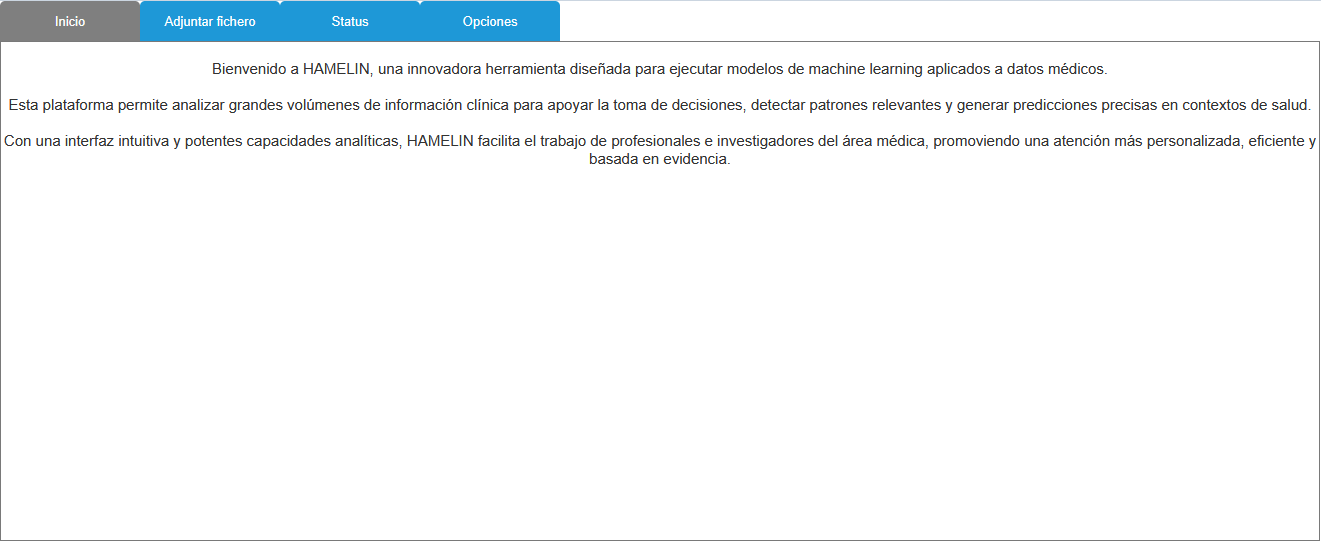
\includegraphics[width=\textwidth]{Figuras/Mockup/Mockup-Inicio.png}
  \caption{Start screen on mockup}
  \label{fig:mockup-inicio}
\end{figure}
    
    \item \textbf{Status}: Automatic dataset exploration, descriptive statistics, missing value analysis.
    \item \textbf{Primary Variable}: Selection of the target variable (outcome).
    \item \textbf{Criteria}: Definition of inclusion and exclusion criteria.
    \item \textbf{Settings}: Configuration of evaluation metrics, missing data strategies, hyperparameter search spaces.
    \item \textbf{Process}: Model training with real-time progress monitoring (Figure \ref{fig:mockup-process}).

\begin{figure}[h]
  \centering
  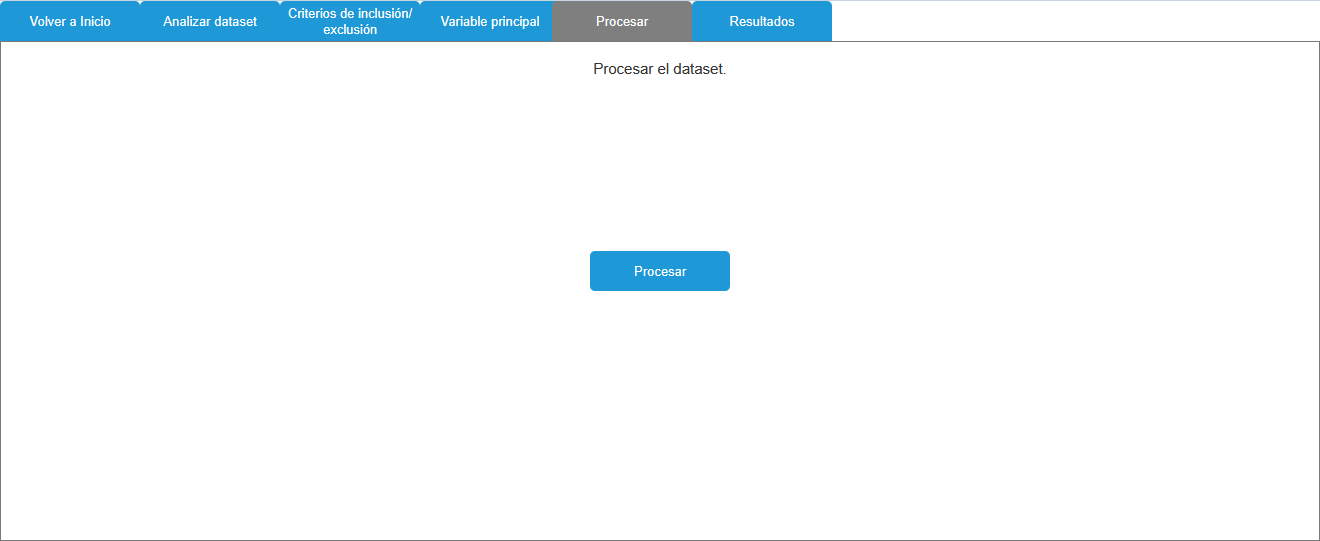
\includegraphics[width=\textwidth]{Figuras/Mockup/Mockup-Process.png}
  \caption{Process screen on mockup}
  \label{fig:mockup-process}
\end{figure}
    
    \item \textbf{Results}: Presentation of model performance, feature importance, predictions (Figure \ref{fig:mockup-results}).
\end{enumerate}

\begin{figure}[h]
  \centering
  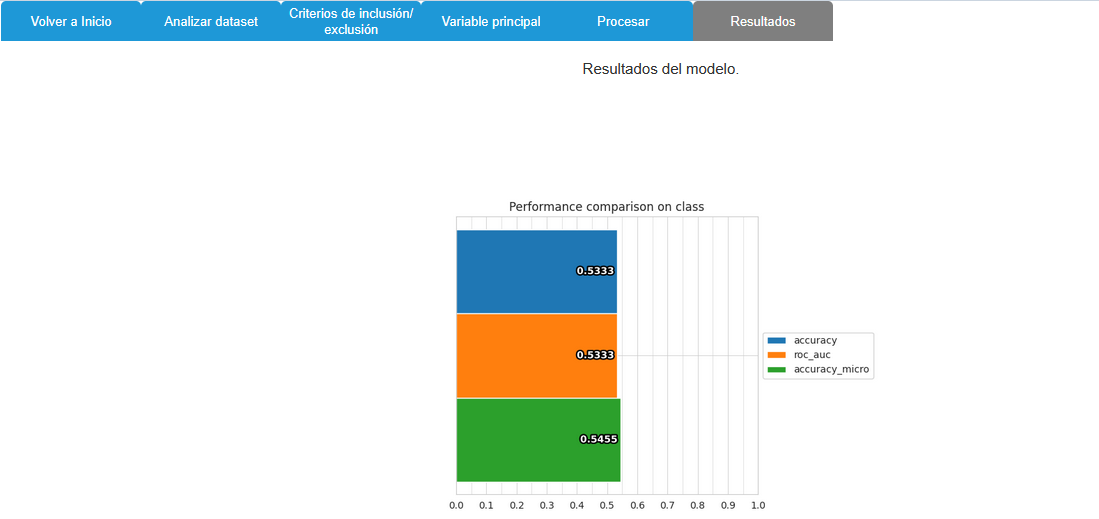
\includegraphics[width=\textwidth]{Figuras/Mockup/Mockup-Resultados.png}
  \caption{Results screen on mockup}
  \label{fig:mockup-results}
\end{figure}

This structure mirrors the logical progression of clinical research: define the question, prepare the data, specify the population, configure the analysis, execute the analysis, interpret the results.

\subsubsection{Mechanisms for protocol-aware interaction}

The mockups incorporated several mechanisms designed to support protocol-aware interaction:

\begin{itemize}
    \item Variable classification: Upon loading a dataset, the system prompts the user to classify variables into categories: demographics, clinical measurements, exposures, outcomes, inclusion/exclusion criteria. This classification informs subsequent steps. For example, variables marked as inclusion/exclusion criteria are used to filter the dataset but are not offered as predictors.

    \item Temporal phase assignment: For longitudinal studies, the system allows users to define protocol phases (screening, baseline, intervention, follow-up) and to assign variables to phases. This prevents data leakage and ensures that predictions use only information available at the time of prediction.

    \item Inclusion/exclusion logic builder: The Criteria tab provides an intuitive interface for specifying inclusion and exclusion rules. Users can define conditions using dropdown menus and logical operators (AND, OR, NOT) without writing code. The system displays the number of individuals included and excluded in real time, allowing users to refine criteria interactively.

    \item Hypothesis-driven variable selection: The Settings tab allows users to mark variables as ``priority'' (based on clinical hypotheses) or ``exploratory'' (to be considered by the system). The \gls{automl} planner gives higher weight to priority variables during feature selection.

    \item Custom evaluation metrics: Users can select from a menu of standard metrics (accuracy, sensitivity, specificity, AUC-ROC, RMSE) and can specify which metric is most important for their research question. The system optimizes models according to the selected metric.

    \item Interpretable visualizations: The Results tab presents model outputs using visualizations familiar to \glspl{crp}: confusion matrices and performance charts.
\end{itemize}

\subsubsection{Feedback and refinement}

The mockups were presented to \glspl{crp} in meetings. Then, \glspl{crp} provided feedback on the overall workflow, terminology and visual design. Key insights included:

\begin{itemize}
    \item Terminology: Terms such as ``primary variable'' (familiar from clinical trial protocols) over ``target variable'' or ``dependent variable'' (statistical jargon).
    \item Context: \glspl{crp} wanted to see metadata about the project (principal investigator, study dates, ethical approvals) before working with data. This led to the addition of a project directory feature.

    \item Flexibility: \glspl{crp} emphasized that variable selection and inclusion criteria vary widely across studies. The system must accommodate this variability rather than imposing a rigid structure.
    
    \item Recruitment tracking: \glspl{crp} requested a feature to track patient recruitment over time and to estimate when the target sample size will be reached. This led to the addition of a recruitment graph in the Status tab.
    
    \item Model transparency: \glspl{crp} wanted to know which \gls{ml} algorithm (Random Forest, Gradient Boosting, etc.) was used for each model, to assess the appropriateness of the method. This information was added to the Results tab.
    
    \item Table 1 generation: \glspl{crp} noted that clinical papers typically include a ``Table 1'' summarizing baseline characteristics of the study population, stratified by outcome or treatment group. They requested that the system generate such a table automatically. This feature was added to the Status tab.
\end{itemize}    

These refinements illustrate the value of iterative, participatory design. By involving \glspl{crp} throughout the design process, the system would align with actual clinical research practices.


\section{Development of the user interfaces of the HGML system}

Building on the mockups and design principles established, this section describes the implementation of the \gls{hamelin} user interface. The interface embodies the \gls{hgml} philosophy by providing \glspl{crp} with meaningful control over the \gls{ml} pipeline while automating computationally intensive tasks.

A key feature of \gls{hgml} is the ability to refine the model iteratively based on initial results. The \gls{hamelin} interface supports this through a reconfiguration mechanism. After reviewing results, users can return to earlier tabs to modify their previous choices. Each time users make a change, the system can re-train the model and updates the results. This iterative process allows \glspl{crp} to explore the modeling space systematically, guided by clinical intuition and domain knowledge.

\subsection{System achitecture}

The \gls{hamelin} system follows a three-layer architecture (Figure \ref{fig:system_architecture}):

\begin{figure}[H]
\centering
\scalebox{0.75}{
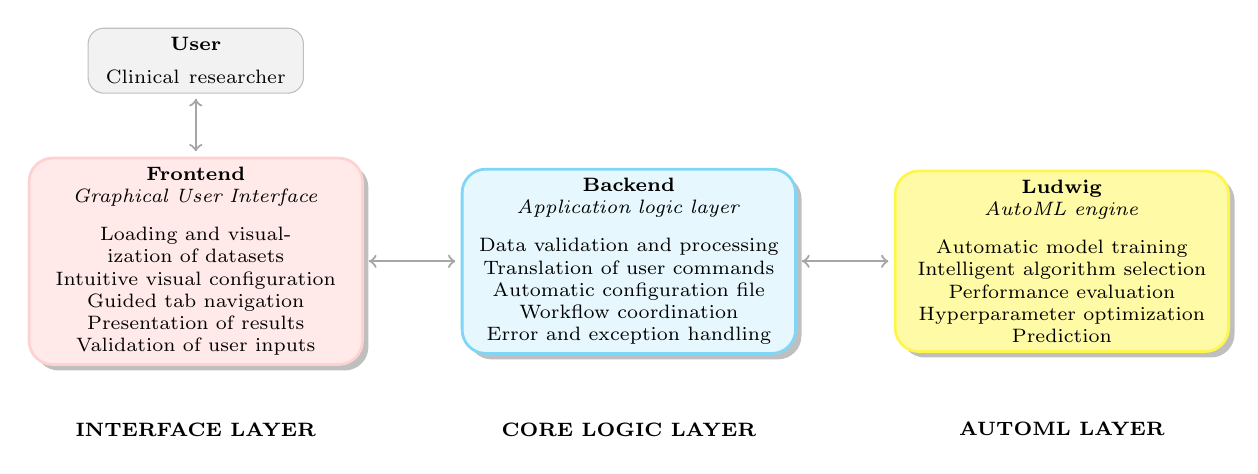
\begin{tikzpicture}[
    node distance=2cm,
    box/.style={
        rectangle,
        draw,
        text width=4cm,
        text centered,
        minimum height=2cm,
        rounded corners=0.3cm,
        drop shadow,
        line width=1pt,
        font=\scriptsize
    },
    frontend/.style={box, fill=pink!35, draw=pink!70},
    backend/.style={box, fill=cyan!10, draw=cyan!50},
    ludwig/.style={box, fill=yellow!35, draw=yellow!70},
    arrow/.style={->, thick, color=gray!70, line width=0.8pt, shorten >=2pt, shorten <=2pt},
    system/.style={
        rectangle,
        draw,
        dotted,
        thick,
        rounded corners=0.4cm,
        color=purple!60,
        line width=1.5pt
    }
]

% Nodos principales (horizontal)
\node[frontend] (frontend) at (0,0) {
    \textbf{Frontend}\\
    \textit{Graphical User Interface}\\[2mm]
    Loading and visualization of datasets\\
    Intuitive visual configuration\\
    Guided tab navigation\\
    Presentation of results\\
    Validation of user inputs
};
\node[backend] (backend) at (5.5,0) {
    \textbf{Backend}\\
    \textit{Application logic layer}\\[2mm]
    Data validation and processing\\
    Translation of user commands\\
    Automatic configuration file\\
    Workflow coordination\\
    Error and exception handling
};
\node[ludwig] (ludwig) at (11,0) {
    \textbf{Ludwig}\\
    \textit{AutoML engine}\\[2mm]
    Automatic model training\\
    Intelligent algorithm selection\\
    Performance evaluation\\
    Hyperparameter optimization\\
    Prediction
};

% Flechas bidireccionales
\draw[arrow] (frontend.east) -- (backend.west);
\draw[arrow] (backend.west) -- (frontend.east);
\draw[arrow] (backend.east) -- (ludwig.west);
\draw[arrow] (ludwig.west) -- (backend.east);

% Usuario
\node[above=0.8cm of frontend.north, 
      rectangle, 
      draw=gray!50, 
      fill=gray!10, 
      text width=2.5cm, 
      text centered,
      rounded corners=0.2cm] (user) {
    \scriptsize \textbf{User}\\
    \scriptsize Clinical researcher
};
\draw[arrow] (user.south) -- (frontend.north);
\draw[arrow] (frontend.north) -- (user.south);

% Etiquetas de capas alineadas y más abajo
\node[below=0.6cm of frontend.south, anchor=north] {\scriptsize \textbf{INTERFACE LAYER}};
\node[below=0.75cm of backend.south, anchor=north] {\scriptsize \textbf{CORE LOGIC LAYER}}; 
\node[below=0.75cm of ludwig.south, anchor=north] {\scriptsize \textbf{AUTOML LAYER}}; 

\end{tikzpicture}
}
\caption{System architecture}
\label{fig:system_architecture}
\end{figure}

\begin{enumerate}
    \item \textbf{Interface Layer}: A \gls{gui} implemented in Python using Qt Designer. Qt Designer was chosen for its simplicity, cross-platform compatibility and ease of integration with Python-based \gls{ml} libraries.

    \item \textbf{Core Logic Layer}: A middleware layer that bridges the \gls{gui} and the \gls{automl} engine. It handles data validation, command translation, configuration file generation, workflow coordination and error handling. This layer is implemented in Python and uses standard libraries for data manipulation (Pandas, NumPy).

    \item \textbf{AutoML Layer}: The Ludwig framework (v0.10.4) serves as the \gls{automl} backend. Ludwig was selected for its declarative, YAML-based configuration, strong community support and ability to handle diverse data types (tabular, text, images). Ludwig automates model training, algorithm selection, hyperparameter optimization and evaluation.
\end{enumerate}

This modular architecture ensures that the interface logic is separated from the \gls{automl} engine. In principle, Ludwig could be replaced with another \gls{automl} framework (e.g., AutoGluon, H2O) without requiring changes to the interface, although some adaptation of the Core Logic Layer would be necessary.

\subsection{Tab-based workflow implementation}

The interface guides users through seven tabs, each corresponding to a distinct phase of the \gls{ml} pipeline.

\subsubsection{Start tab: Project creation and dataset loading}

The Start tab is the entry point to the system. Users begin by creating a new project or opening an existing one. When creating a project, users provide metadata:

\begin{itemize}
    \item \textbf{Project name}: A short identifier.
    \item \textbf{Principal investigator}: The lead researcher.
    \item \textbf{Study type}: Patient registry, observational study or clinical trial.
    \item \textbf{Date of first patient}: The start date of data collection.
    \item \textbf{Ethical approvals}: Reference numbers for ethical review board approvals.
    \item \textbf{Objectives}: A brief description of the research question.
\end{itemize}

This metadata is stored in a project directory and displayed throughout the session, providing context for all subsequent decisions.

Users then load a dataset by selecting a CSV file. The system performs basic validation (checking for empty columns, duplicate rows, unsupported data types) and displays a preview of the data. If validation fails, the system provides actionable error messages (e.g., ``Column `Age' contains non-numeric values. Please correct the file and reload.'').

\subsubsection{Status tab: Automatic dataset exploration}

Upon successful loading, the system automatically generates descriptive statistics and visualizations. The Status tab displays (Figure \ref{fig:interface-status}):

\begin{figure}[h]
  \centering
  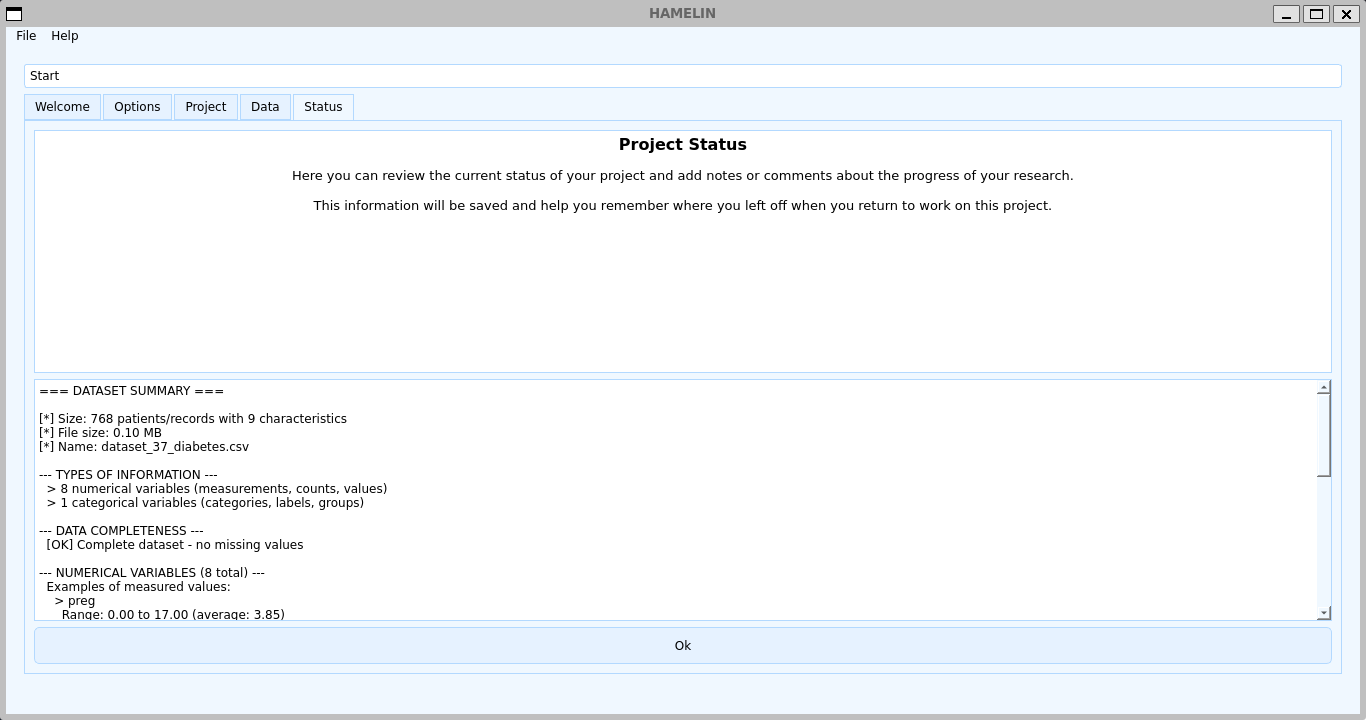
\includegraphics[width=\textwidth]{Figuras/Interface/interface-status.png}
  \caption{Status}
  \label{fig:interface-status}
\end{figure}

\begin{itemize}
    \item \textbf{Sample size}: Number of rows (patients) and columns (variables).
    \item \textbf{Variable types}: Counts of numeric, categorical and date variables.
    \item \textbf{Missing data summary}: Percentage of missing values per variable, visualized as a heatmap.
    \item \textbf{Univariate distributions} (To be completed.): Histograms for numeric variables, bar charts for categorical variables.
    \item \textbf{Recruitment timeline} (To be completed.): If the dataset includes a date column indicating when each patient was added, the system plots cumulative recruitment over time and projects when the target sample size will be reached (based on linear extrapolation).
    \item \textbf{Table 1} (To be completed.): A summary table showing baseline characteristics, stratified by the outcome variable (if already selected) or by treatment group (if specified). This table follows the conventions of clinical research publications.
\end{itemize}

The Status tab serves two purposes. First, it familiarizes users with the dataset, helping them identify potential issues (outliers, data entry errors, unexpected distributions). Second, it provides information that informs subsequent decisions (e.g., which variables have too much missing data to be useful).

\subsubsection{Primary Variable tab: Target selection}

The Primary Variable tab prompts users to select the outcome variable (target) for the predictive model. The system lists all variables and allows users to choose one. Upon selection, the system automatically detects the task type:

\begin{itemize}
    \item \textbf{Binary classification}: If the variable has two unique values (e.g., ``Yes''/``No'', 0/1).
    \item \textbf{Multi-class classification}: If the variable has more than two unique values and is categorical.
    \item \textbf{Regression}: If the variable is numeric and continuous.
\end{itemize}

The system displays the distribution of the target variable and flags potential issues (e.g., severe class imbalance in classification tasks). Users can proceed to the next tab or return to the Status tab to explore the data further.

\subsubsection{Criteria tab: Inclusion and exclusion logic}

The Criteria tab allows users to define the analysis population by specifying inclusion and exclusion criteria. The interface provides a rule builder with the following components (Figure \ref{fig:interface-criteria1}, Figure \ref{fig:interface-criteria2}):

\begin{figure}[h]
  \centering
  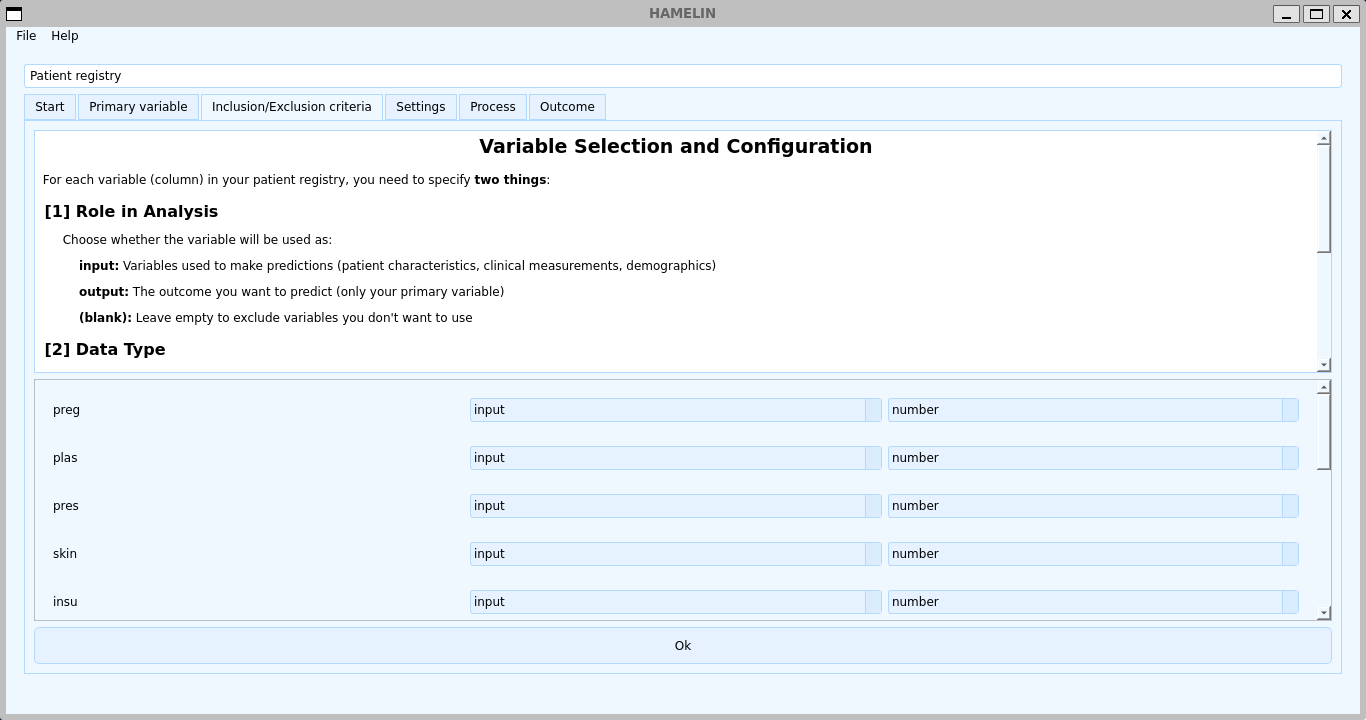
\includegraphics[width=\textwidth]{Figuras/Interface/interface-criteria.png}
  \caption{Criteria 1}
  \label{fig:interface-criteria1}
\end{figure}

\begin{figure}[h]
  \centering
  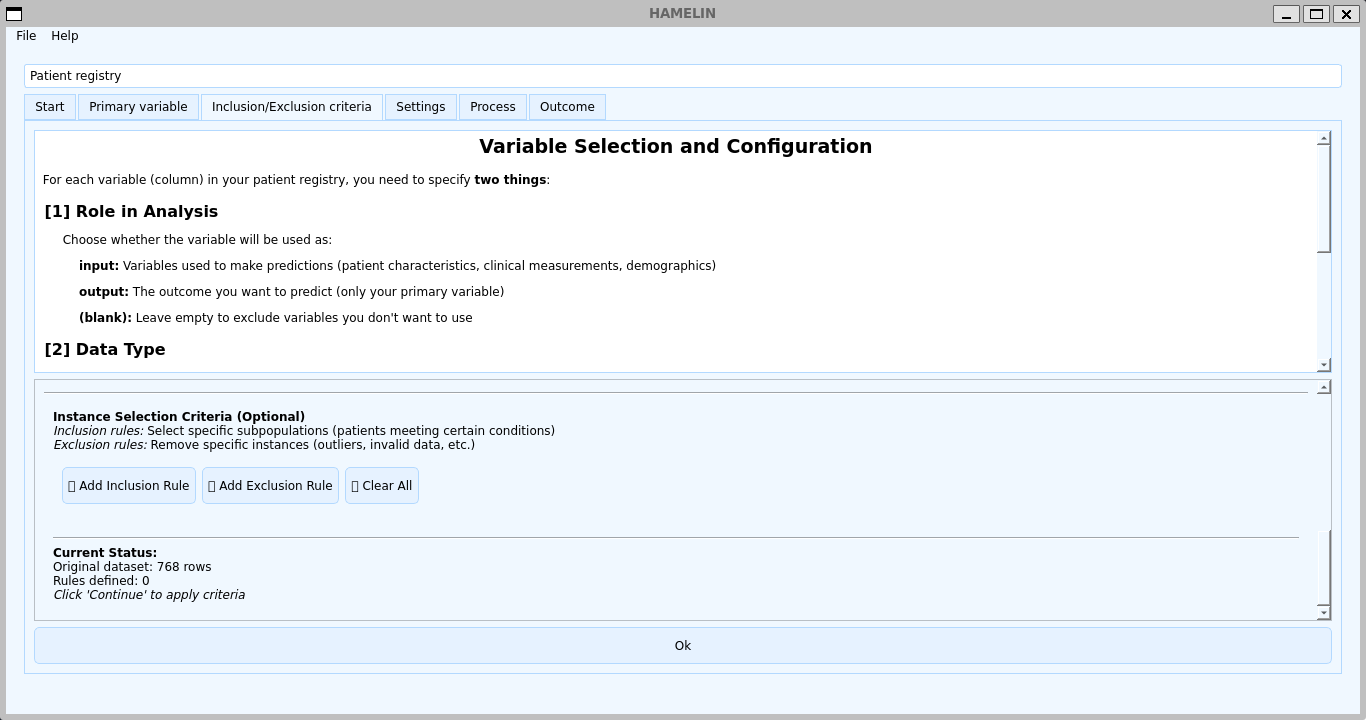
\includegraphics[width=\textwidth]{Figuras/Interface/interface-criteria2.png}
  \caption{Criteria 2}
  \label{fig:interface-criteria2}
\end{figure}

\begin{itemize}
    \item \textbf{Variable selector}: A dropdown menu listing all variables in the dataset.
    \item \textbf{Operator selector}: Dropdown menus for comparison operators (=, $\neq$, <, $\leq$, >, $\geq$, contains, does not contain).
    \item \textbf{Value input}: A text field or dropdown (for categorical variables) where users specify the threshold or category.
    \item \textbf{Logical connectors}: Buttons for AND, OR, NOT, allowing users to combine multiple conditions.
\end{itemize}

Users can add, edit or remove rules interactively. Once satisfied, users apply the criteria, and the system filters the dataset accordingly. The filtered dataset is used for all subsequent steps.

This feature addresses a critical gap in existing \gls{automl} tools, which provide no native support for defining study populations.

% Revisar
\subsubsection{Settings tab: Configuration of metrics, missing data strategies and hyperparameters}

The Settings tab allows users to configure several aspects of the \gls{ml} pipeline:

\textbf{CSV separator}: Users can specify the field separator used in CSV files. Supported delimiters include comma (,), semicolon (;) and backslash (\textbackslash), ensuring correct parsing of datasets generated from different sources or regional configurations.

\textbf{Evaluation metrics}: Users select which metrics to compute (accuracy, precision, recall, F1-score, AUC-ROC for classification; MAE, RMSE, $R^2$ for regression). They also specify which metric should be used to select the best model during hyperparameter optimization.

\textbf{Missing data handling}: Users choose a strategy for each variable with missing data:

\begin{itemize}
    \item \textbf{fill\_with\_const}: Replace missing values with a user-specified constant value.
    \item \textbf{fill\_with\_mode}: Replace missing values with the most frequent value in the column.
    \item \textbf{fill\_with\_mean}: Replace missing values with the mean of the column (numeric features only).
    \item \textbf{fill\_with\_false}: Replace missing values with false (binary features only).
    \item \textbf{bfill}: Replace missing values with the next valid value from subsequent rows (backward fill).
    \item \textbf{ffill}: Replace missing values with the previous valid value from preceding rows (forward fill, useful for longitudinal data).
    \item \textbf{drop\_row}: Remove the entire row from the dataset if this column is missing.
\end{itemize}

For output features (the target variable), the default strategy is always \textit{drop\_row}, as Ludwig cannot train on cases where the ground truth is unknown. However, this can be overridden if required by the research design.

\textbf{Time-dependent}: Users indicate whether the attached data has a temporal structure. When enabled, the system treats observations as ordered in time, allowing the application of time-aware preprocessing steps such as forward/backward filling and ensuring that data splitting, validation, and model evaluation respect temporal causality. This setting is particularly relevant for longitudinal, sequential, or time-series data, where ignoring temporal dependencies could lead to information leakage or misleading performance estimates.

\textbf{Runtime}: Users can adjust the maximum training time of the model. This setting allows balancing computational cost and model performance by limiting the duration of hyperparameter optimization and training.

\subsubsection{Process tab: Model training with real-time monitoring}

Once the pipeline is configured, users proceed to the Process tab and initiate training by clicking a ``Train Model'' button. The system translates the user's choices into a Ludwig configuration file (YAML format) and this executes the training process.

During training, the Process tab displays:

    Progress bar: Indicating the percentage of the hyperparameter search completed.
    Current model: The algorithm and hyperparameters being evaluated.
    Best model so far: The algorithm, hyperparameters and performance metric of the best model found to date.
    Estimated time remaining: Based on the time taken for previous iterations.

This real-time feedback reassures users that the system is working and provides transparency into the AutoML process.

Training can take several minutes, depending on dataset size and the complexity of the search space. Users can pause or cancel training at any time.

\subsubsection{Results tab: Interactive presentation of model performance}

Upon completion of training, the system presents results in the Results tab. The presentation is tailored to the task type (Figure \ref{fig:interface-confusionmatrix}, Figure \ref{fig:interface-performance}):

\begin{figure}[h]
  \centering
  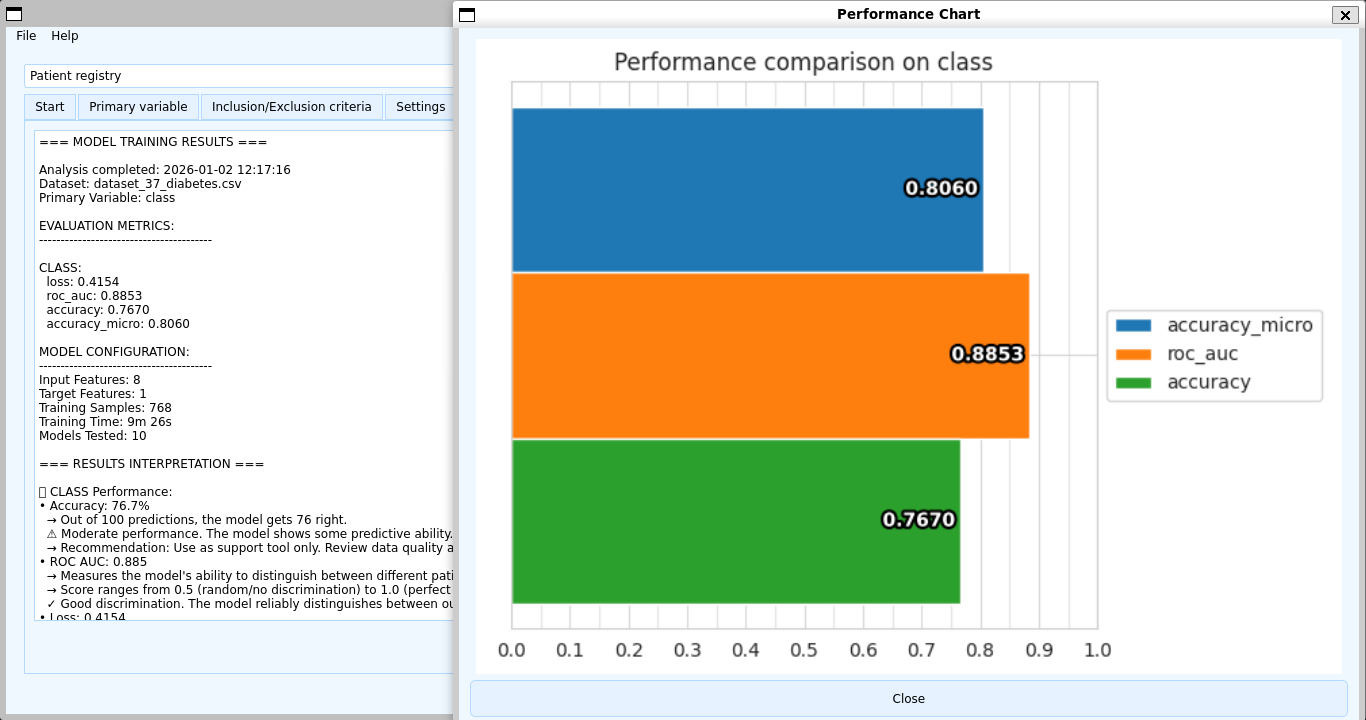
\includegraphics[width=\textwidth]{Figuras/Interface/interface-performance.png}
  \caption{Performance comparison}
  \label{fig:interface-performance}
\end{figure}

\begin{figure}[h]
  \centering
  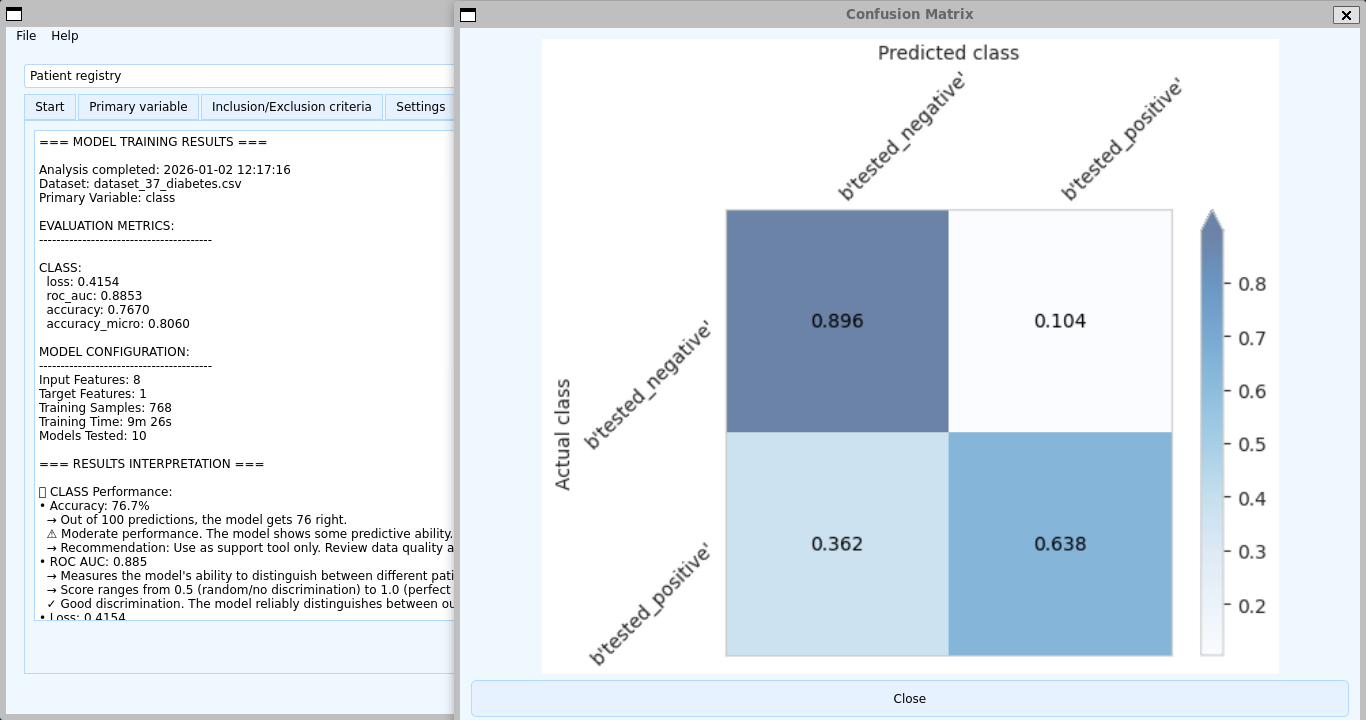
\includegraphics[width=\textwidth]{Figuras/Interface/interface-confusionmatrix.png}
  \caption{Confusion matrix}
  \label{fig:interface-confusionmatrix}
\end{figure}

For classification tasks, results are presented through a confusion matrix visualised as a heatmap, which displays true positives, false positives, true negatives and false negatives. In addition, a table reports the main performance metrics: accuracy, precision, recall, F1-score and AUC-ROC.

For regression tasks, performance is summarised in a table including MAE, RMSE and 
$R^2$.




\bibliographystyle{plain}
\bibliography{refs/example.bib}
\nocite{*}

\end{document}
